
\noindent This chapter covers the following ideas.

\begin{enumerate}
	\item Explain Hooke's Law in regards to mass-spring systems, where there is an external force. Construct and solve differential equations which represent this physical model, with or without the presence of a damper and be able to interpret how solutions change based on changes in the model. 
	\item Understand the theory which relates solutions of homogeneous linear ODE's to non homogeneous ODEs. 
	\item Use the method of undetermined coefficients  to solve non homogeneous linear ODEs.
	\item Explain Kirchhoff's voltage law, Ohm's law, and how to model electrical circuits using 2nd order non homogeneous linear ODEs.  Illustrate how results about circuits can be translated into results about mass-spring systems.
\end{enumerate}

The problems below come from Schaum's Outlines \textit{Differential Equations} by Richard Bronson. If you are struggling with a topic from the preparation problem set, please use this list as a guideline to find related practice problems.

\begin{center}
\begin{tabular}{|l|c|l|l|l|l|}
\hline
Concept&Sec&Suggestions&Relevant Problems\\ \hline
Theory&8&21,65&21-23,65-67\\ \hline
Undetermined Coef&11&1,2,3,8,10,24,26,34,36,41,46,47,48&All\\ \hline
IVP&13&1,7,14&1,3,7,8,10,11,14\\ \hline
Applications&7&19,76&19-22,71-81\\ \hline
Applications&14&10,11,13,14,17,46,50,51,52,54,57&9-18,44-65\\ \hline
\end{tabular}
\end{center}




\end{document}


Start with the big picture.  Where are we headed. Show them that we'll be learning to solve ODE's that are non homogeneous. 
Maybe have them develop the ODEs for mass-spring systems that are driven.  Also have them develop an ODE for an electrical network. 

To introduce, start by solving a matrix equation.  Solve Ax=0, and then Ax=b (in the same problem).  Ask them what the difference is.  Have them create their own example next (make sure there is more than one solution).  What do they notice.

Then have the prove general facts about matrices.  If x and y are both solutions to Ax=b, then x-y is a solution to Ax=0.  (maybe change the variables). 
Now we jump to ODEs.  Have them solve a simple one, using Laplace transforms.  Have them check if the same pattern holds.
Have them prove the general pattern. If y_1 and y_2 are solutions, then their difference solves the homogeneous ODE.  
This gives us a tool.  All we need to do is find a single solution, and then we're done.




\section{An example - Hooke's Law}
Second order non homogeneous linear ODEs occur in mass-spring systems when there is an outside force, such as a machine applying pressure, bumps in a road causing vertical motion on shock absorbers, etc. If a spring is involved in some kind of moving object, then forces will be applied to the spring from outside the system. If we let $r(t)$ represent the external force (sometimes called the driving, or input force), then the sum of the forces acting on the spring is $-ky-cy'+r(t)$, so Newton's 2nd law $F=ma = my''$ gives the differential equation $my''=-cy'-ky+r(t)$, or $my''+cy'+ky=r(t)$.  The solution $y(t)$ is called the output or response of the system to the driving force.  Solving such a system in general can be a difficult task.  We will discuss the ideas behind solving such ODE's in general first, and then focus on a special case where the driving force is periodic of the form $r(t)=F_0\cos \omega t$. Near the end of this book in the Fourier series chapter, we will show how the solutions to this simple periodic force can give solutions to any period force. 

\section{Theory}
If $y_p$ is a particular solution to a non homogeneous linear ODE, and $y_c$ is a solution to the corresponding homogeneous linear ODE, then $y_c+y_p$ is a solution to the non homogeneous linear ODE. We call $y_p$ a particular solution, and $y_c$ we call a complementary solution. If $y_1$ and $y_2$ are two particular solutions to a non homogeneous linear ODE, then the difference $y_1-y_2$ is a solution to the corresponding homogeneous ODE. This is because if you put both of them into the ODE, you will get out the same driving force, so if you subtract them, you will get out out zero. This means that $y_2=y_1+y_c$ for some solution $y_c$ of the homogeneous linear ODE. This shows the following.
\begin{theorem}
A general solution to a non homogeneous linear ODE is $y=y_c+y_p$ where $y_p$ is a particular solution to the ODE and $y_c$ is a general solution of the corresponding homogeneous linear ODE. 
\end{theorem}
To solve a non homogeneous linear ODE, we first find a single solution $y_p$ to the ODE and then add to it a general solution of the corresponding homogeneous ODE. If we can guess a particular solution and we know how to find homogeneous solutions (from the previous chapter), then we can find a general solution of a non homogeneous ODE. The existence and uniqueness theorems apply to non homogeneous ODEs.

\begin{example} Consider the non homogeneous ODE $y''+4y = 8x$. The function $y_p=2x$ is a particular solution to this ODE, since $y_p''=0$ and then $4(2x)=8x$ (before this chapter ends you will learn how to discover $y_p=2x$, but for now let's just use it to illustrate an idea). Removing the driving force $8x$ gives the corresponding homogeneous ODE $y''+4y=0$.  The characteristic equation of this homogeneous ODE is $\lambda^2+4=0$, whose solutions are $\lambda =\pm 2i$.  A general solution to the homogeneous ODE is $y_c = c_1 \cos 2x +c_2\sin 2x$. A general solution to the non homogeneous ODE is found by simply summing the particular $y_p$ and complementary $y_c$ solutions, giving $$y = y_p+y_c = 2x+y_c = c_1 \cos 2x +c_2\sin 2x.$$
\end{example}

\section{Method of Undetermined Coefficients}
If a linear ODE can be written in the form $y''+ay'+by=r(x)$, where $r(x)$ is an exponential function, a polynomial, a cosine or sine, or sums or products of such functions, then we will be able to find particular solutions to the ODE by making educated guesses. 
The idea is to notice that derivatives of these types of functions involve functions similar to themselves.  To find a particular solution, we chose as our guess a function which is very similar to $r(x)$, which has unknown coefficients which we then determine by taking derivatives of our guess, substituting them into our ODE, and then solving for the unknown coefficients.  Table~\ref{undeterminedcoefficient} illustrates the type of guesses that should be made based on what form $r(x)$ takes.
\begin{table}
\begin{center}
\begin{tabular}{|l|l|}
\hline
Form of $r(x)$ & Guess for $y_p$\\\hline\hline
$ke^{ax}$ & $Ce^{ax}$\\\hline
$kx^n$ & $K_n x^n + K_{n-1}x^{n-1}+\cdots+K_1 x^1 +K_0$\\\hline
$k\cos(\omega x)$ or $k\sin(\omega x)$ & $K\cos(\omega x)+M\sin(\omega x)$\\\hline
$ke^{ax}\cos(\omega x)$ or $ke^{ax}\sin(\omega x)$ & $Ke^{ax}\cos(\omega x)+Me^{ax}\sin(\omega x)$\\\hline
\end{tabular}
\caption{Method of Undetermined Coefficients. For every term in the driving force $r(x)$ of the form on the left, your guess $y_p$ for the particular solution should contain the terms on the right.}
\label{undeterminedcoefficient}
\end{center}
\end{table}
There are three key rules needed to use this table to make appropriate guesses, the product rule, modification rule, and sum rule. 
\begin{itemize}

\item \textbf{Product Rule}: If $r(x)$ contains a term which is the produce of terms in Table~\ref{undeterminedcoefficient}, then include in $y_p$ a product of the corresponding guesses, giving each term in the product it's own undetermined coefficient.
\item \textbf{Modification Rule}: Select a single term in $r(x)$. After applying the product rule (if needed), if the guess from Table~\ref{undeterminedcoefficient} contains a term which is a solution to the corresponding homogeneous ODE, then multiply the entire guess by $x$. If your guess still contains a term which is a solution to the homogeneous ODE, then keep multiplying by $x$ until no terms are solutions to the homogeneous ODE. This requires that we start each problem by solving the corresponding homogeneous linear ODE. 
\item \textbf{Sum Rule}: If $r(x)$ is a sum of functions in Table~\ref{undeterminedcoefficient}, then make an appropriate guess for each term in $r(x)$, and choose for $y_p$ the sum of the guesses (combining coefficients when the same term appears more than once).
\end{itemize}
Following are a few examples of how this method works. These ideas can be discovered using Laplace transforms, but the details to do this are more involved than just making an educated guess and then showing that your guess is correct. When we learn about systems of ODEs, we will use matrices and the matrix exponential to organize all this work and show how the method of undetermined coefficients really comes from simple integration on matrices.

\begin{example}
To solve $y''+5y'+4y=3$, we first solve the homogeneous ODE $y''+5y'+4y=0$. The characteristic equation $\lambda^2+5\lambda+4=(\lambda+4)(\lambda+1)=0$ has roots $\lambda=-4,-1$, which means the complementary solution is $y_c = c_1e^{-4x}+c_2e^{-x}$. Since the driving force is a constant, we guess the particular solution $y_p=K_0$ with unknown coefficient $K_0$.  We put $y_p, y_p' = 0$ and $y_p'' = 0$ into the ODE to obtain the equation $0+0+4(K_0)=3,$ or $K_0=3/4$. A general solution to the non homogeneous ODE is $y=y_c+y_p = c_1e^{-4x}+c_2e^{-x} + 3/4$.
\end{example}

\begin{example}
To solve $y''+5y'+4y=3x^2$, we first solve the homogeneous ODE $y''+5y'+4y=0$. As in the previous example, the characteristic equation $\lambda^2+5\lambda+4=(\lambda+4)(\lambda+1)=0$ has roots $\lambda=-4,-1$, which means the complementary solution is  $y_c = c_1e^{-4x}+c_2e^{-x}$.  Because the driving force is a parabola, we choose $y_p=K_2x^2+K_1x+K_0$ for unknown coefficients $K_2, K_1,K_0$.  We put $y_p, y_p' = 2K_2x+K_1,$ and $y_p'' = 2K_2$ into the ODE to obtain the equation $$2K_2+5(2K_2x+K_1)+4(K_2x^2+K_1x+K_0)=3x^2.
$$ \marginpar{{\begin{tabular}{c|c|c|c|}
&$x^2$&$x$&1\\ \hline\hline
$y''$&0 & 0 & $2K_2$\\
$5y'$&0 & $10K_2$ & $5K_1$\\
$4y$&$4K_2$ & $4K_1$ & $4K_0$\\ \hline
$r(t)$ &3 & 0 & 0
\end{tabular}

You can organize your work by placing the coefficients of each power of $x$ in their corresponding column.  Then the sum of each column must match the coefficient of the driving force.
}}To solve for the unknown constants, we factor the equation (grouping each power of $x$ - the table on the side can simplify  this) to obtain 
$$ (4K_2)x^2  + ( 10K_2 +4K_1)x + ( 2K_2 +5 K_1 + 4 K_0)= 3x^2. $$ The only way for the polynomial on the left to equal the polynomial on the right is if the coefficients of each power of $x$ are the same on both sides.  This means that we have to solve the linear system (back to linear algebra) $4K_2=3, 10K_2 +4K_1=0,2K_2 +5 K_1 + 4 K_0=0$.  Using back substitution, we have $K_2=3/4, K_1 = -15/8, K_0=63/32$. So the general solution to the non homogeneous ODE is $y=y_c+y_p = c_1e^{-4x}+c_2e^{-x} + 3/4x^2-15/8x+63/32$.
\end{example}

\begin{example}
To solve $y''+6y'+9y=5e^{-3x}$, we first solve the homogeneous linear ODE $y''+6y'+9y=0$. The characteristic equation $\lambda^2+6\lambda+9=(\lambda+3)(\lambda+3)=0$ has a double root $\lambda=-3$.  Hence we get $y_c = c_1e^{-3x}+c_2xe^{-3x}$. As a guess for a particular solution, we choose $y_p=Ke^{-3x}$ for an unknown coefficient $K$. However, this is a solution in $y_c$, so we use the modification rule and multiply by $x$ twice to obtain $y_p=Kx^2e^{-3x}$ as our guess. We put $y_p, y_p' = 2 Kx{e^{-3x}}-3K{x}^{2}{e^{-3x}}$ and $y_p'' = 2K{e^{-3x}}-12Kx{e^{-3x}}+9K{x}^{2}{e^{-3x}}$ into the ODE to obtain the equation 
$$ {e^{-3x}}(2K-12Kx+9K{x}^{2})+6{e^{-3x}}(2 Kx-3K{x}^{2})+9(Kx^2e^{-3x})=5e^{-3x} .$$
We can organize our work in table form, as shown on the side. 
\marginpar{{\begin{tabular}{c|c|c|c|}
&$x^2e^{-3x}$&$xe^{-3x}$&$e^{-3x}$\\ \hline\hline
$y''$& $9K$ & $-12K $ & $2K$ \\
$6y'$&$-18K$ & $12 K$ & \\
$9y$&$9K$ &  & \\ \hline
$r(t)$ &0 & 0 & 5
\end{tabular}
}} 
Equating coefficients of like terms on both sides gives us two trivial equations $0=0$ -- this reduction will happen whenever repeated roots appear. The last equation simplifies to give $2 K{e^{-3x}} = 5e^{-3x}$, and so $K=5/2$. Hence, the general solution to the non homogeneous ODE is $y=y_c+y_p = c_1e^{-3x}+c_2xe^{-3x} + (5/2)x^2e^{-3x}$.

\end{example}

\begin{example}
To solve the ODE $y''+y=4\cos x+e^{2x}\sin 3x$, we first solve the homogeneous linear ODE $y''+y=0$, which has general solution $y=c_1\cos x +c_2\sin x$. Since $\cos(x)$ is a solution of the homogeneous ODE, we choose $x(A\cos x+B\sin x)$ as a term in $y_p$ (modify both the cosine and sine term). The term $e^{2x}\sin 3x$ yields the guess 
$Ce^{2x}\cos 3x+ D e^{2x} \sin 3x$. Using the sum rule we add these two guesses together to obtain our final guess for a particular solution $$y_p= x(A\cos x+B\sin x) + Ce^{2x}\cos 3x+ D e^{2x} \sin 3x.$$  The first derivative is (using the product rule for derivatives) 
\begin{align*}
y_p'=& x(-A\sin x+B\cos x) +(A\cos x+B\sin x) \\
&-3Ce^{2x}\sin 3x+ 2Ce^{2x}\cos 3x+ 3 D e^{2x} \cos 3x + 2D e^{2x} \sin 3x\\ 
=& (A+Bx)\cos x +(B-Ax)\sin x \\
&+e^{2x}( (2C+3D)\cos 3x  + (2D-3C)\sin 3x ).
\end{align*}
The second derivative is 
\begin{align*}
y_p''=&-(A+Bx)\sin x +(B)\cos x +(B-Ax)\cos x-A\sin x \\
&+e^{2x}( -3(2C+3D)\sin 3x  + 3(2D-3C)\cos 3x )\\
&+2e^{2x}( (2C+3D)\cos 3x  + (2D-3C)\sin 3x )\\
=& (2B-Ax)\cos x +(-2A-Bx)\sin x \\
&+
 e^{2x} ( (-5C+12D) \cos 3x  + (-12C-5D)\sin  3x ).
\end{align*}
In table form we write
\begin{center}
\begin{tabular}{c|c|c|c|c|c|c|}
&$\cos x$ & $\sin x$ &$x\cos x$ & $x\sin x$ & $e^{2x}\cos 3x$ & $e^{2x}\sin 3x$\\\hline\hline
$y$& &  &$A$ & $B$ & $C$ & $D$\\
$y'$&$A$ & $B$ &$B$ & $-A$ & $2C+3D$ & $2D-3C$\\
$y''$&$2B$ & $-2A$ &$-A$ & $-B$ & $-5C+12D$ & $-12C-5D$\\
\end{tabular}
\end{center}
Putting $y_p,y_p',$ and $y_p''$ into the ODE $y''+y=4\cos x+e^{2x}\sin 3x$ (eliminating the middle row), and placing the terms in table form (to simplify organization), we have \marginpar{With practice you can start skipping steps and speed up organization by using a table to factor your derivatives.}  
\begin{center}
\begin{tabular}{c|c|c|c|c|c|c|}
&$\cos x$ & $\sin x$ &$x\cos x$ & $x\sin x$ & $e^{2x}\cos 3x$ & $e^{2x}\sin 3x$\\\hline\hline
$y''$&$2B$ & $-2A$ &$-A$ & $-B$ & $-5C+12D$ & $-12C-5D$\\
$y$& &  &$A$ & $B$ & $C$ & $D$\\\hline
$r(t)$&$4$ & 0 & 0& 0 & 0 & 1\\
\end{tabular}
\end{center}
Summing the columns and equating coefficients gives the 4 non trivial equations $2B=4$, $-2A=0$, $-4C+12D=0$, $-12C-4D=1$ (notice that two of the equations vanished, which always happens when the modification rule is used).  These four equations immediately shows that $B=2$ and $A=0$. Using Cramer's rule gives $C=-3/40$ and $D=-1/40$. The general solution is $$y=y_c+y_p= c_1\cos x +c_2\sin x+2x\sin x -\frac{3}{40}e^{2x}\cos 3x-\frac{1}{40} e^{2x} \sin 3x.$$
\end{example}






\section{Hooke's Law Again}
We now return to the mass-spring system where the driving force $r(t)$ is not zero in the differential equation $my''+cy'+ky=r(t)$. We will examine a periodic (with period $\frac{2\pi}{\omega}$) driving force of the form $r(t)=F_0\cos \omega t$ for some constants $F_0$ and $\omega$. The number $\omega$ is called the angular frequency. We will give a general solution to this ODE, and then explore how $F_0$ and $\omega$ can influence the solution.  In particular, we will discover how resonance (large oscillations) can occur. The collapse of the Tacoma Narrows bridge in 1940 provides a visual illustration of how resonance must be accounted for in mechanical design, as the forces from wind generated vorticies pushed and pulled on the bridge structure at just the right frequency to cause the bridge to collapse ({\footnotesize see wikipedia or Billah, K.; R. Scanlan (1991). ``Resonance, Tacoma Narrows Bridge Failure, and Undergraduate Physics Textbooks''}). 

The quadratic equation tells us that the zeros of the characteristic equation $m\lambda^2+c\lambda+k=0$ are 
$$\lambda = \frac{-c\pm \sqrt{c^2-4mk}}{2m}.$$
If $c\neq 0$, then the complementary solution will not contain a $\cos \omega x$ or $\sin \omega x$, which means that the modification rule will not be needed when selecting $y_p$. If $c=0$, then the roots are $\ds\pm\sqrt{\frac{k}{m}}$, so as long as $\sqrt{k/m}\neq \omega$ we do not need to worry about the modification rule.  We'll assume for the moment that the modification rule does not need to be used, and then consider the case $\omega=\sqrt{k/m}$ afterwards.

Using the method of undetermined coefficients, we guess the solution 
$$y_p(t) = a\cos\omega t+b\sin\omega t. $$  
Differentiation gives 
$$y_p'(t) = -a\omega\sin\omega t+b\omega\cos\omega t \text{ and } y_p''(t) = -a\omega^2\cos\omega t-b\omega^2\sin\omega t.$$  Substitution into the ODE gives
$m(-a\omega^2\cos\omega t-b\omega^2\sin\omega t)+c(-a\omega\sin\omega t+b\omega\cos\omega t)+k(a\cos\omega t+b\sin\omega t)=F_0\cos \omega t$. Factoring the left side gives $(-am\omega^2+bc\omega+ak)\cos\omega t+(-bm\omega^2-ac\omega+bk)\sin\omega t=F_0\cos \omega t$ (the table on the right organizes our work). Hence we have the linear system 
\marginpar{{\begin{center}
\begin{tabular}{c|c|c|}
&$\cos \omega t$ & $\sin \omega t$ \\\hline\hline
$my''$&$-am\omega^2 $ & $-bm\omega^2 $ \\
$cy'$ &$bc\omega $   &$-ac\omega $  \\
$ky$  &$ak$ &$bk$  \\\hline
$r(t)$&$F_0$ & 0 \\
\end{tabular}
\end{center}}}
$$\begin{cases}
(k-m\omega^2)a+bc\omega = F_0\\
-ac\omega+(k-m\omega^2)b=0
\end{cases} \rightarrow
\begin{bmatrix}
(k-m\omega^2)&c\omega\\
-c\omega& (k-m\omega^2)
\end{bmatrix}
\begin{bmatrix}
a\\b
\end{bmatrix}
=\begin{bmatrix}
F_0\\0
\end{bmatrix}
,$$ where $a$ and $b$ are our unknown constants. Cramer's rule gives the solution to this system, by computing
\begin{align*}
a=\frac{\begin{vmatrix}F_0&c\omega\\
0& (k-m\omega^2)
\end{vmatrix}}{\begin{vmatrix}(k-m\omega^2)&c\omega\\
-c\omega& (k-m\omega^2)
\end{vmatrix}}=\frac{F_0(k-m\omega^2)}{(k-m\omega^2)^2+c^2\omega^2},
\\ 
b=\frac{\begin{vmatrix}(k-m\omega^2)&F_0\\
-c\omega& 0
\end{vmatrix}}{\begin{vmatrix}(k-m\omega^2)&c\omega\\
-c\omega& (k-m\omega^2)
\end{vmatrix}}=\frac{F_0 c\omega }{(k-m\omega^2)^2+c^2\omega^2}.
\end{align*}
This gives a particular solution to the ODE to which we add $y_c(t)$ to find the general solution. If you make the substitution $\omega_0=\sqrt{k/m}$ (or $k=m\omega_0^2$), then the solution becomes (you do not need to memorize this, however you should know how to derive it)
$$a=F_0\frac{m(\omega_0^2-\omega^2)}{m^2(\omega_0^2-\omega^2)^2+c^2\omega^2}\ \ \ \ \ \ b=F_0\frac{c\omega}{m^2(\omega_0^2-\omega^2)^2+c^2\omega^2}.$$
This gives us a general formula for studying the motion of a mass spring system which is driven by an external periodic force.

\begin{observation}
When $c>0$, the homogeneous solution to a damped mass-spring system will involve exponentials which approach 0 as $t\to \infty$. This means that $y_c\to o$ as $t\to \infty$, so the solution $y=y_c+y_p$ tends to follow the (stable) solution $y_p$ as $t\to\infty$. We call $y_c$ the transient solution as it dies out, and $y_p$ the steady state solution as it is the solution left after significant passage of time. The particular solution has the same period (hence the same frequency) as the driving force (recall that frequency is defined as 1/period). In other words, this means that after a reasonable amount of time, the solution to a damped mass-spring system with a sinusoidal driving force will become a harmonic oscillation with frequency matching the frequency of the driving force.
\end{observation}

\begin{observation}
If $c=0$ and $w\neq\omega_0$ (remember $\omega_0=\sqrt{k/m}$), then $\ds a=\frac{F_0}{m(\omega_0^2-\omega^2)}$ and $b=0$. Hence we can write $$y(t) = y_c+y_p=C\cos(\omega_0 t-\delta)+\frac{F_0}{m(\omega_0^2-\omega^2)}\cos\omega t.$$  This is the superposition of two harmonic oscillations with differing frequencies. 
\marginpar{{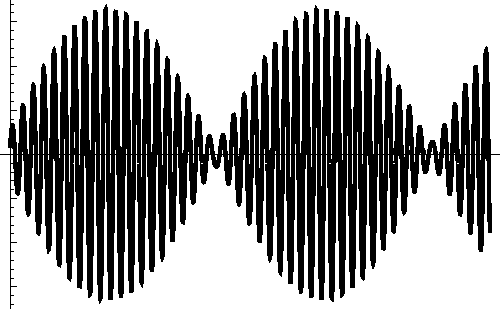
\includegraphics[width=\marginparwidth]{06-Non-Homogeneous-ODEs/resonnance}
\\
This is a typical graph of a solution with resonance. In this example, $w = 2$, $m=1.1$, $c\approx 0$, and $k=4$.  Since $\omega_0=\sqrt{4/1.1}\approx 2=\omega$, the quantity $\ds\frac{F_0}{m(\omega_0^2-\omega^2)}$ has a small denominator, which results in large periodic oscillations. If the oscillations are too large, they will destroy the system.
}}
As $\omega\to\omega_0$, the amplitude of the particular solution approaches infinity, and so we have extremely large oscillations (often called resonance). When the two frequencies are extremely close together, resonance can result in huge oscillations which can tear apart a mechanical system almost instantly. Notice in the picture on the right how the solution  

As a side note, the word frequency is used in different ways in different places. Always attach either circular or natural to the word frequency to convey the correct idea.
\begin{itemize}
\item The circular (angular) frequency, is $\omega_0 = \sqrt{k/m}$ (radians per second).
\item The natural frequency is $f = \frac{\omega_0}{2\pi}$ (hertz).
\end{itemize}
The period (distance from one peak to the next) is always interpret as the reciprocal of the natural frequency, $T=1/f$.
\end{observation}

\begin{observation}
If $c=0$ and $w=\omega_0 = \sqrt{k/m}$, then the modification rule applies and we use the method of undetermined coefficients to find $a$ and $b$ in $y_p=t(a\cos(\omega_0 t)+b\sin(\omega_0 t))$ (notice the $t$ in front). The solution is 
$$y_p(t) = \frac{F_0}{2m\omega_0}t\sin(\omega_0 t).$$ The $t$ in this solution causes the amplitude of the vibration to grow,  increasing without bound in a linear fashion. In this setting, any system will destroy itself as the oscillations will become too large to physically keep the system together. 

\marginpar{{
%\begin{figure}[h]
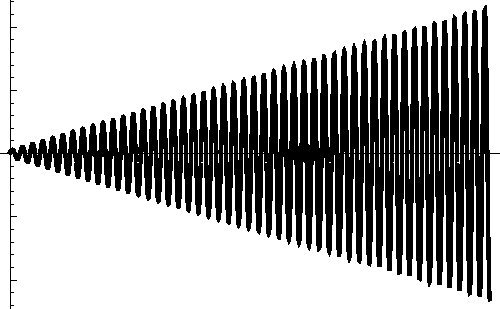
\includegraphics[width=\marginparwidth]{06-Non-Homogeneous-ODEs/growing-oscillation}

When $\omega_0=\omega$ and friction is negligible, a system will oscillate with an amplitude that grows without bound. Beware of this situation, as any mechanical system which undergoes this kind of oscillation will self destruct. 
%\end{figure}
}}
Anytime a mechanical system is built, the builders must study the internal frequencies of the system and make sure that they will not match external forces applied to the system. Soldiers marching across a bridge have collapsed a bridge in the past, so now it is common for soldiers to stop marching and shuffle across a bridge to prevent it from collapsing. The Tacoma Narrows bridge collapsed from forces due to resonance. Engineers must pay attention to both internal and external forces, making sure to avoid resonance.  
\end{observation}

\section{Electric circuits} (This section is largely a summary of page 116 from Schaum's Outlines.)
Kirchoff's Voltage law states that the voltage (electromotive force) impressed on a closed loop is equal to the sum of the voltage drops across the other elements of the loop. We use the expression $I(t)$ to represent the current in a loop. The following table illustrates summarizes the three types of voltage drops we will study.
\begin{center}
\begin{tabular}{|l|l|l|}
\hline
Component & Voltage drop & Other\\\hline
Resistor & $RI$ & Ohm's law, where $R$ is in ohms\\\hline
Inductor & $LI' = L(dI/dt)$ & $L$ is in henrys\\\hline
Capacitor& $Q/C$ & $Q$ is in coulombs, $C$ in farads.\\\hline
\end{tabular}
\end{center}
Here $Q$ is the charge on the capacitor, related to the current by $I(t)=\frac{dQ}{dt}$, or $Q=\int I(t) dt$.


\marginpar{{
\begin{center}
\renewcommand{\myscale}{.3}
\begin{tikzpicture}[scale=\myscale,inner sep=1pt]
%\draw[help lines,step=1cm] (0,0) grid (12,6);

%Source - like a battery
\node[label=right:$E$] at (0,3) 
{{\begin{tikzpicture}[scale=\myscale]
%	\useasboundingbox (-.5,-3) rectangle (.5,3);
	\draw (0,0) circle (1cm);
	\draw (.3,.5) -- (-.3,.5);
	\draw (0,.2) -- (0,.8);
	\draw (.3,-.5) -- (-.3,-.5);
	\draw (0,1) -- (0,3);
	\draw (0,-1) -- (0,-3);
	\end{tikzpicture}
}};

%Resistor
\node[label=right:$R$] at (6,3) 
{{\begin{tikzpicture}[scale=\myscale]
%	\useasboundingbox (0,-3) rectangle (0,3);
	\draw (0,-3) -- ++(0,1.8) -- ++(.5,.2) 
		-- ++(-1,.4) -- ++(1,.4)
		-- ++(-1,.4) -- ++(1,.4)
		-- ++(-1,.4) -- ++(.5,.2)
		-- ++(0,1.8) ;
	\end{tikzpicture}
}};

%Straight Path
%\node at (3,6) 
%{{\begin{tikzpicture}[scale=\myscale,rotate=90]
%	\draw (0,-3) -- (0,3);
%	\end{tikzpicture}
%}};

%Arrow to represent Current
\node[label=right:$i$] at (0,5) 
{{\begin{tikzpicture}[scale=\myscale,rotate=0]
	\filldraw (0,.4) -- (-.2,-.4) -- (0,-.3) -- (.2,-.4);
	\end{tikzpicture}
}};

%Loops
\node[label=above:$L$] at (3,6) 
{{\begin{tikzpicture}[scale=\myscale,rotate=90]
	\useasboundingbox (-.5,-3) rectangle (.5,3);
	\draw (0,-3) -- ++(0,1.5) 
	.. controls+(15:.2) and +(-90:.25) .. ++(.5,.4) 
	.. controls+(90:.25) and +(-15:.2) .. ++(-.5,.4) 
	.. controls+(-15:-.2) and +(90:.1) .. ++(-.5,-.05) 
	.. controls+(-90:.1) and +(15:-.2) .. ++(.5,-.05) 
	.. controls+(15:.2) and +(-90:.25) .. ++(.5,.4) 
	.. controls+(90:.25) and +(-15:.2) .. ++(-.5,.4) 
	.. controls+(-15:-.2) and +(90:.1) .. ++(-.5,-.05) 
	.. controls+(-90:.1) and +(15:-.2) .. ++(.5,-.05) 
	.. controls+(15:.2) and +(-90:.25) .. ++(.5,.4) 
	.. controls+(90:.25) and +(-15:.2) .. ++(-.5,.4) 
	.. controls+(-15:-.2) and +(90:.1) .. ++(-.5,-.05) 
	.. controls+(-90:.1) and +(15:-.2) .. ++(.5,-.05) 
	.. controls+(15:.2) and +(-90:.25) .. ++(.5,.4) 
	.. controls+(90:.25) and +(-15:.2) .. ++(-.5,.4) 
	-- (0,3);
	\end{tikzpicture}
}};


%Capacitor
\node[label=above:$C$] at (3,0) 
{{\begin{tikzpicture}[scale=\myscale,rotate=90]
%	\useasboundingbox (0,-3) rectangle (0,3);
	\draw (0,-3) -- ++(0,2.8) 
		-- ++(.5,0) -- ++(-1,0) 
		++(0,.4) -- ++(1,0)
		-- ++(-.5,0) -- ++(0,2.8);
	\end{tikzpicture}
}};


\end{tikzpicture}

\\
An $RLC$-circuit
\\
\vspace{.2in}
\renewcommand{\myscale}{.3}
\begin{tikzpicture}[scale=\myscale,inner sep=1pt]
%\draw[help lines,step=1cm] (0,0) grid (12,6);

%Source - like a battery
\node[label=right:$E$] at (0,3) 
{{\begin{tikzpicture}[scale=\myscale]
%	\useasboundingbox (-.5,-3) rectangle (.5,3);
	\draw (0,0) circle (1cm);
	\draw (.3,.5) -- (-.3,.5);
	\draw (0,.2) -- (0,.8);
	\draw (.3,-.5) -- (-.3,-.5);
	\draw (0,1) -- (0,3);
	\draw (0,-1) -- (0,-3);
	\end{tikzpicture}
}};

%Resistor
\node[label=right:$R$] at (6,3) 
{{\begin{tikzpicture}[scale=\myscale]
%	\useasboundingbox (0,-3) rectangle (0,3);
	\draw (0,-3) -- ++(0,1.8) -- ++(.5,.2) 
		-- ++(-1,.4) -- ++(1,.4)
		-- ++(-1,.4) -- ++(1,.4)
		-- ++(-1,.4) -- ++(.5,.2)
		-- ++(0,1.8) ;
	\end{tikzpicture}
}};

%Straight Path
\node at (3,6) 
{{\begin{tikzpicture}[scale=\myscale,rotate=90]
	\draw (0,-3) -- (0,3);
	\end{tikzpicture}
}};

%Arrow to represent Current
\node[label=above:$i$] at (3,6) 
{{\begin{tikzpicture}[scale=\myscale,rotate=-90]
	\filldraw (0,.4) -- (-.2,-.4) -- (0,-.3) -- (.2,-.4);
	\end{tikzpicture}
}};

%Inductor
%\node[label=above:$L$] at (3,6) 
%{{\begin{tikzpicture}[scale=\myscale,rotate=90]
%	\useasboundingbox (-.5,-3) rectangle (.5,3);
%	\draw (0,-3) -- ++(0,1.5) 
%	.. controls+(15:.2) and +(-90:.25) .. ++(.5,.4) 
%	.. controls+(90:.25) and +(-15:.2) .. ++(-.5,.4) 
%	.. controls+(-15:-.2) and +(90:.1) .. ++(-.5,-.05) 
%	.. controls+(-90:.1) and +(15:-.2) .. ++(.5,-.05) 
%	.. controls+(15:.2) and +(-90:.25) .. ++(.5,.4) 
%	.. controls+(90:.25) and +(-15:.2) .. ++(-.5,.4) 
%	.. controls+(-15:-.2) and +(90:.1) .. ++(-.5,-.05) 
%	.. controls+(-90:.1) and +(15:-.2) .. ++(.5,-.05) 
%	.. controls+(15:.2) and +(-90:.25) .. ++(.5,.4) 
%	.. controls+(90:.25) and +(-15:.2) .. ++(-.5,.4) 
%	.. controls+(-15:-.2) and +(90:.1) .. ++(-.5,-.05) 
%	.. controls+(-90:.1) and +(15:-.2) .. ++(.5,-.05) 
%	.. controls+(15:.2) and +(-90:.25) .. ++(.5,.4) 
%	.. controls+(90:.25) and +(-15:.2) .. ++(-.5,.4) 
%	-- (0,3);
%	\end{tikzpicture}
%}};


%Capacitor
\node[label=above:$C$] at (3,0) 
{{\begin{tikzpicture}[scale=\myscale,rotate=90]
%	\useasboundingbox (0,-3) rectangle (0,3);
	\draw (0,-3) -- ++(0,2.8) 
		-- ++(.5,0) -- ++(-1,0) 
		++(0,.4) -- ++(1,0)
		-- ++(-.5,0) -- ++(0,2.8);
	\end{tikzpicture}
}};


\end{tikzpicture}

\\
An $RC$-circuit
\\
\vspace{.2in}
\renewcommand{\myscale}{.3}
\begin{tikzpicture}[scale=\myscale,inner sep=1pt]
%\draw[help lines,step=1cm] (0,0) grid (12,6);

%Source - like a battery
\node[label=right:$E$] at (0,3) 
{{\begin{tikzpicture}[scale=\myscale]
%	\useasboundingbox (-.5,-3) rectangle (.5,3);
	\draw (0,0) circle (1cm);
	\draw (.3,.5) -- (-.3,.5);
	\draw (0,.2) -- (0,.8);
	\draw (.3,-.5) -- (-.3,-.5);
	\draw (0,1) -- (0,3);
	\draw (0,-1) -- (0,-3);
	\end{tikzpicture}
}};

%Resistor
\node[label=right:$R$] at (6,3) 
{{\begin{tikzpicture}[scale=\myscale]
%	\useasboundingbox (0,-3) rectangle (0,3);
	\draw (0,-3) -- ++(0,1.8) -- ++(.5,.2) 
		-- ++(-1,.4) -- ++(1,.4)
		-- ++(-1,.4) -- ++(1,.4)
		-- ++(-1,.4) -- ++(.5,.2)
		-- ++(0,1.8) ;
	\end{tikzpicture}
}};

%Straight Path
\node at (3,0) 
{{\begin{tikzpicture}[scale=\myscale,rotate=90]
	\draw (0,-3) -- (0,3);
	\end{tikzpicture}
}};

%Arrow to represent Current
\node[label=above:$i$] at (3,0) 
{{\begin{tikzpicture}[scale=\myscale,rotate=90]
	\filldraw (0,.4) -- (-.2,-.4) -- (0,-.3) -- (.2,-.4);
	\end{tikzpicture}
}};

%Inductor
\node[label=above:$L$] at (3,6) 
{{\begin{tikzpicture}[scale=\myscale,rotate=90]
	\useasboundingbox (-.5,-3) rectangle (.5,3);
	\draw (0,-3) -- ++(0,1.5) 
	.. controls+(15:.2) and +(-90:.25) .. ++(.5,.4) 
	.. controls+(90:.25) and +(-15:.2) .. ++(-.5,.4) 
	.. controls+(-15:-.2) and +(90:.1) .. ++(-.5,-.05) 
	.. controls+(-90:.1) and +(15:-.2) .. ++(.5,-.05) 
	.. controls+(15:.2) and +(-90:.25) .. ++(.5,.4) 
	.. controls+(90:.25) and +(-15:.2) .. ++(-.5,.4) 
	.. controls+(-15:-.2) and +(90:.1) .. ++(-.5,-.05) 
	.. controls+(-90:.1) and +(15:-.2) .. ++(.5,-.05) 
	.. controls+(15:.2) and +(-90:.25) .. ++(.5,.4) 
	.. controls+(90:.25) and +(-15:.2) .. ++(-.5,.4) 
	.. controls+(-15:-.2) and +(90:.1) .. ++(-.5,-.05) 
	.. controls+(-90:.1) and +(15:-.2) .. ++(.5,-.05) 
	.. controls+(15:.2) and +(-90:.25) .. ++(.5,.4) 
	.. controls+(90:.25) and +(-15:.2) .. ++(-.5,.4) 
	-- (0,3);
	\end{tikzpicture}
}};


%Capacitor
%\node[label=above:$C$] at (3,0) 
%{{\begin{tikzpicture}[scale=\myscale,rotate=90]
%	\draw (0,-3) -- ++(0,2.8) 
%		-- ++(.5,0) -- ++(-1,0) 
%		++(0,.4) -- ++(1,0)
%		-- ++(-.5,0) -- ++(0,2.8)
%	\end{tikzpicture}
%}};


\end{tikzpicture}

\\
An $RL$-circuit
\end{center}}}
In a circuit  with one resistor, one inductor, and one capacitor (an $RLC$ circuit), if the electromotive force is $E(t)$, then Kirchoff's Voltage law gives the integro-differential equation 
$$L I'+ RI+ \frac{1}{C}Q(t) =E(t) \quad \text{or}\quad L I'+ RI+ \frac{1}{C}\int I(t) dt = E(t).$$  
Differentiating both sides removes the integral and gives
$$L I''+ RI'+ \frac{1}{C}I(t) = E'(t),$$ which is a 2nd order non homogeneous linear differential equation with constant coefficients. 
If the electromotive force is sinusoidal (such as $E(t) = E_0\sin(\omega t)$), then we can solve this differential equation to find the current exactly the same way we did in the last section. Notice however that initial conditions will most often be given in terms of initial charge $Q(0)$ and initial current $I(0)$.  To solve the differential equation, you will have to use the first equation $ L I'(t)+ RI(t)+ \frac{1}{C}Q(t) =E(t)$ to obtain a value for $I'(0)$

Due to time constraints, I will let you read the examples in the text for examples involving specific $RLC$, $RC$, and $RL$ circuits. When working with $RC$-circuits, you differentiate both sides to obtain a first order ODE, and initial conditions are generally given as initial charge.  When working with an $RL$-circuit, you don't need to differentiate $E(t)$, and the initial current is generally given for initial conditions. One key observation to make is that when you are given initial conditions for the charge and current, you use these to find initial conditions for the current's derivative. Even when $Q(0)=0$ and $I(0)=0$, we may find that $I'(0)\neq 0$. Use the equation involving $Q$ to find $I'(0)$. (Problem 14.13 provides an excellent example of how this can occur.) 

\section{Comparing the two models - saving money}

Mechanical models are expensive to build.  Electrical models are fairly simple to build and measure.  If you need to create a mechanical system, it may prove beneficial financially to start with an electrical model. Engineers spend another semester on this idea in system dynamics.  Hydraulic systems are also very closely related. In bridging between mechanical and electrical systems, we compare the following variables. 

\begin{center}
\begin{tabular}{|c|c|c|c|c|c|}
\hline
Mechanical System&$m$&$c$&$k$&$r(t)=F_0\cos\omega t$&$y(t)$\\\hline
Electrical System&$L$&$R$&$1/C$&$E'(t) = E_0\omega\cos\omega t$&$I(t)$\\
\hline
\end{tabular}
\end{center}

Solving a problem in one system (either mechanical or electrical) can provide useful results in the other.  

